Este capítulo descreve a definição do banco de dados Cassandra operando em \textit{cluster}, assim como características, funcionalidades o porquê da sua escolha e como realizar avaliações neste banco. 

Cassandra é um sistema de banco de dados baseado na abordagem NoSQL (\textit{Not only Structure Query Language}), do tipo chave/valor. Nesse tipo de banco de dados, os dados são identificados através de uma chave \cite{Silva}.
A principal promessa do Cassandra é de prover um sistema de armazenamento distribuído, altamente escalável e eventualmente consistente. Para garantir essas promessas,
foram unidas características de dois sistemas NoSQL, o BigTable do Google e o Dynamo da Amazon.
Esse sistema foi criado no Facebook em 2008, por Avinash Lakshman e Prashant Malik e foi bastante usado pelo próprio Facebook para tornar a busca de mensagens mais robusta. 


Um sistema de banco de dados somente pode abranger dois itens entre consistência, disponibilidade e tolerância a partições. Entre essas três
opções, o Cassandra garante disponibilidade dos dados e tolerância a partições \cite{Silva}.

Para garantir que um grande volume de dados seja tratado de forma rápida e eficiente, o Cassandra possui por trás uma arquitetura bastante robusta e complexa. Essa arquitetura é composta por diversos sistemas distribuídos que garantem que cada parte do sistema funcione corretamente.

Quando uma requisição de leitura ou escrita é feita, qualquer nó do \textit{cluster} pode tratá-la. Através da chave, o nó que atendeu a requisição consegue saber quais nós possuem informações dos dados. O sistema então aguarda até que um número configurado de réplicas, chamado \textit{quorum}, responder com o dado, no caso de leitura; ou responder com uma confirmação, no caso de uma escrita.

\section{Particionamento de Dados}
O \textit{cluster} do Cassandra é organizado em um anel, sendo que cada nó do anel possui um intervalo de valores determinado. Os dados são divididos entre os diversos nós através de um \textit{hashing} da chave identificadora desses dados. Esse \textit{hash} gera um valor que então determina, através do intervalo de cada nó do anel, qual dessas máquinas será responsável por esse dado. Essas máquinas responsáveis pelos dados são chamadas de coordenadoras.
Essa divisão dos nós em anel facilita a adição e remoção de nós no \textit{cluster}. Quando um nó é adicionado ou removido no \textit{cluster}, somente os vizinhos desse nó são afetados. Isso garante que o sistema seja bastante escalável, já que a adição de um nó no \textit{cluster} não afeta o funcionamento de todo o sistema.

\section{Replicação de Dados}
A replicação no Cassandra é utilizada para garantir a alta disponibilidade dos dados. Cada dado é encontrado em N nós do \textit{cluster}, sendo que N é um fator de replicação configurável. O coordenador do nó (definido anteriormente) é o responsável por replicar os dados entre os N-1 nós. Essa réplica feita pelo coordenador pode ser feita de três formas diferentes: \textit{Rack Unaware}, \textit{Rack Aware} e \textit{Datacenter Aware}. No modo \textit{Rack Unaware}, o coordenador simplesmente seleciona os próximos N-1 nós do anel. Nos modos \textit{Rack Aware} e \textit{Datacenter Aware}, é utilizado um sistema externo que elege um líder, que tem como função avisar cada nó que se conecta ao \textit{cluster} a faixa de valores do anel que ele será uma réplica. A Figura \ref{fig:gravacaoCassandra} tem uma representação desse anel, onde cada nó é responsável por armazenar dados cuja chave primária esta dentro de uma faixa de valor. Essa chave primária determina em qual nó os dados serão escritos e é utilizando ela que o sistema faz cópia dos dados e os distribui entre um grupo de nós. 

    \begin{figure}[htb]
    \centering
    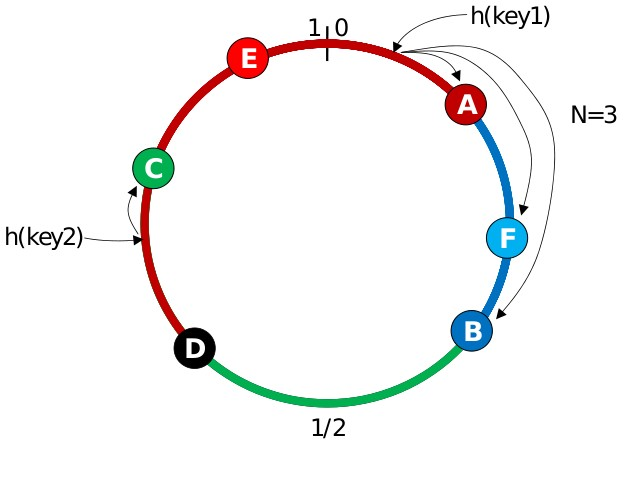
\includegraphics[scale=0.5]{imagens/cassandra.png}
    \caption{Exemplo de gravação de dados no Cassandra} \cite[p. 3]{Silva}
    \label{fig:gravacaoCassandra}
    \end{figure}
    
    
\section{Cassandra: o porquê de sua escolha}

A criação de um \textit{cluster} Cassandra é fácil de ser configurada e ampliada, os dados podem ficar distribuídos de acordo com o planejamento de utilização. Além disso, sua arquitetura é escalável e dependendo da demanda é possível aumentar o número de nós do \textit{cluster}, sem que haja interrupção do serviço.

O Cassandra também conta com menor concorrência, ou seja, o(s) \textit{webservice(s)} não acessam um único nó, ele(s) podem acessar qualquer nó a qualquer momento, fazendo com o que o sistema como um todo tenha melhor desempenho e aumento da disponibilidade.


\section{Avaliação do Cassandra}

Utilizou-se o JMeter e o CassJMeter para testar os diferentes cenários propostos para o Cassandra no projeto Maritaca \cite{DenisSheahan2012}.

\subsection{Criando um Plano de Teste}

Plano de teste é o componente básico para a criação de qualquer \textit{script} (.jmx) utilizando o JMeter e descreve uma série de passos que a ferramenta irá executar quando executar os testes \cite{De2013}. Ao plano de teste são adicionados os demais componentes pertinentes aos testes que serão executados. Os principais componentes estão ilustrados na Figura \ref{fig:plantest} e são:

\begin{itemize}
\item Thread (\textit{users}) - Grupo de usuários: representação de um grupo de usuário executando determinada(s) solicitação(ões);
\item Elemento de configuração: representação dos itens de configuração, que pode ser Cassandra \textit{Properties}, \textit{Schema Properties}, Configuração dos dados CSV, entre outros;
\item Testador: representação de uma solicitação, que pode ser HTTP, FTP, Cassandra \textit{Put}, Cassandra \textit{Get}, Cassandra \textit{Composite Put}, Cassandra \textit{Composite Get}, Cassandra \textit{Batch Put}, Cassandra \textit{Delete}, entre outras e
\item Ouvintes: elementos que capturam os resultados gerados pelo plano de testes e apresenta-os em um determinado formato, com vinculo ou não a um plano de testes.

\end{itemize}

   \begin{figure}[htb]
    \centering
    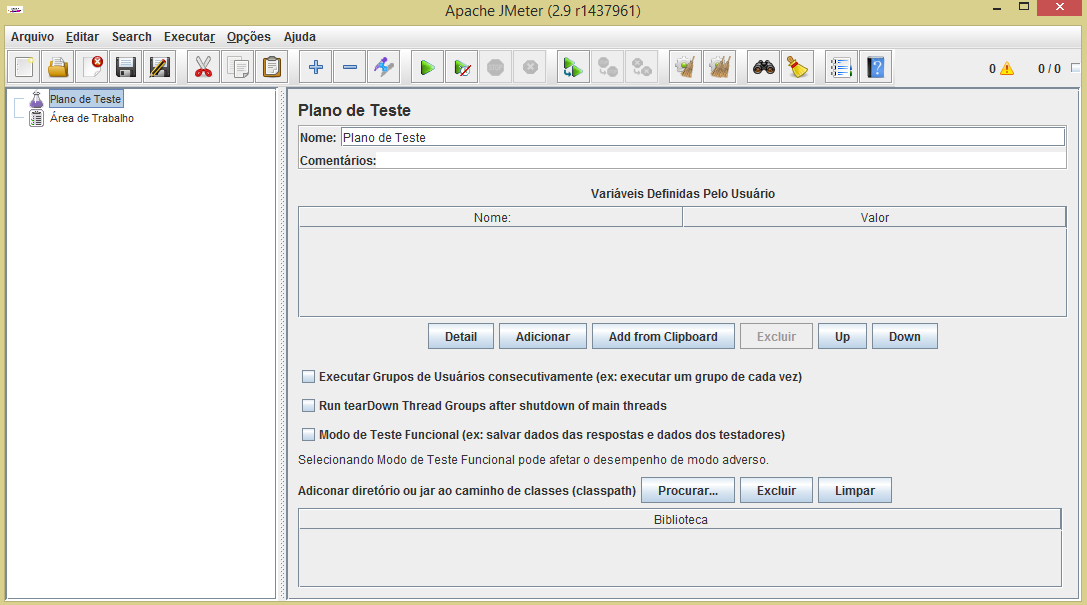
\includegraphics[scale=0.5]{imagens/plantest.png}
    \caption{Exemplo de plano de teste}
    \label{fig:plantest}
    \end{figure}

\subsection{Adicionando usuários virtuais}

Para simular as ações dos usuários o JMeter permite a adição de um componente chamado Grupo de Usuários. Este componente agrega todos os demais elementos necessários para a execução dos testes, controlando as ações de pseudos usuários no
sistema. Para adicioná-lo ao Plano de Teste basta acionar: Editar/Adicionar/\textit{Threads(Users)}/Grupo de Usuários. Conforme ilustra a Figura \ref{fig:grupodeusuarios}.

   \begin{figure}[htb]
    \centering
    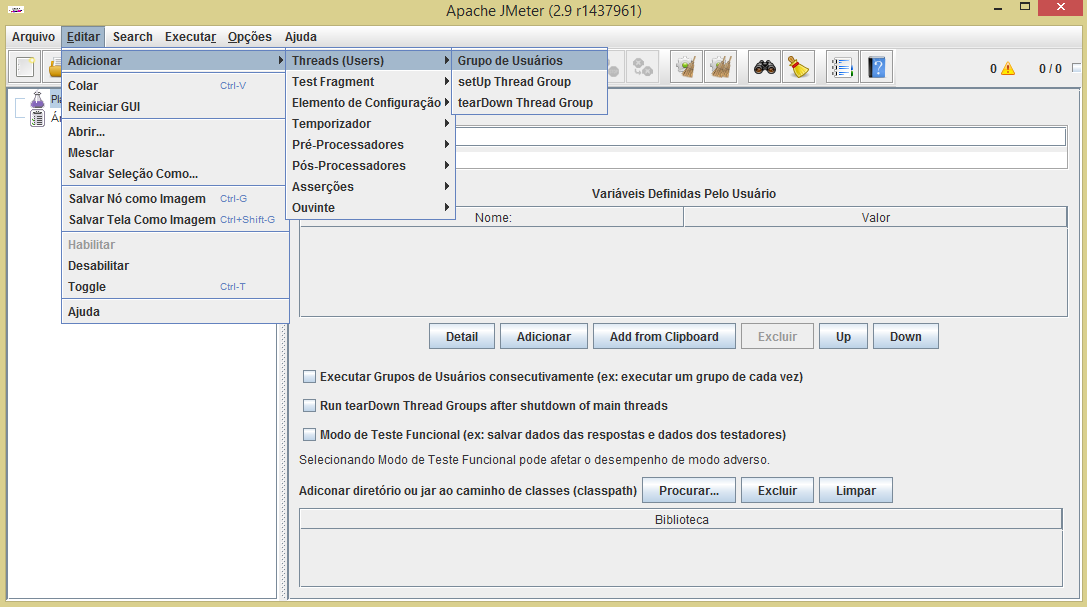
\includegraphics[scale=0.5]{imagens/usergroup.png}
    \caption{Criando grupo de usuários}
    \label{fig:grupodeusuarios}
    \end{figure}


Uma das funcionalidades da tela Grupo de Usuários é controlar o número de usuários que acessaram o sistema. Com isso, foram efetuados testes variando a quantidade de usuários entre 100 e 5000.

\subsection{Configurando acesso ao \textit{cluster} Cassandra}

Para conseguir acessar o \textit{cluster} Cassandra é necessário adicionar o item Cassandra \textit{Properties} aos Elementos de Configuração. Com este elemento é possível definir quais nós do \textit{cluster} serão acessados e em qual porta, qual tipo de interface será utilizada para enviar requisições aos nós do \textit{cluster}, qual o nome do \textit{cluster}, em qual \textit{keyspace} serão realizados os testes, qual o máximo de conexões por nó e qual o tipo de consistência de leitura e escrita serão utilizadas. O caminho para adicionar o item Cassandra \textit{Properties} é: Editar/Adicionar/Elemento de Configuração, conforme Figura \ref{fig:cassandraproperties}.


   \begin{figure}[htb]
    \centering
    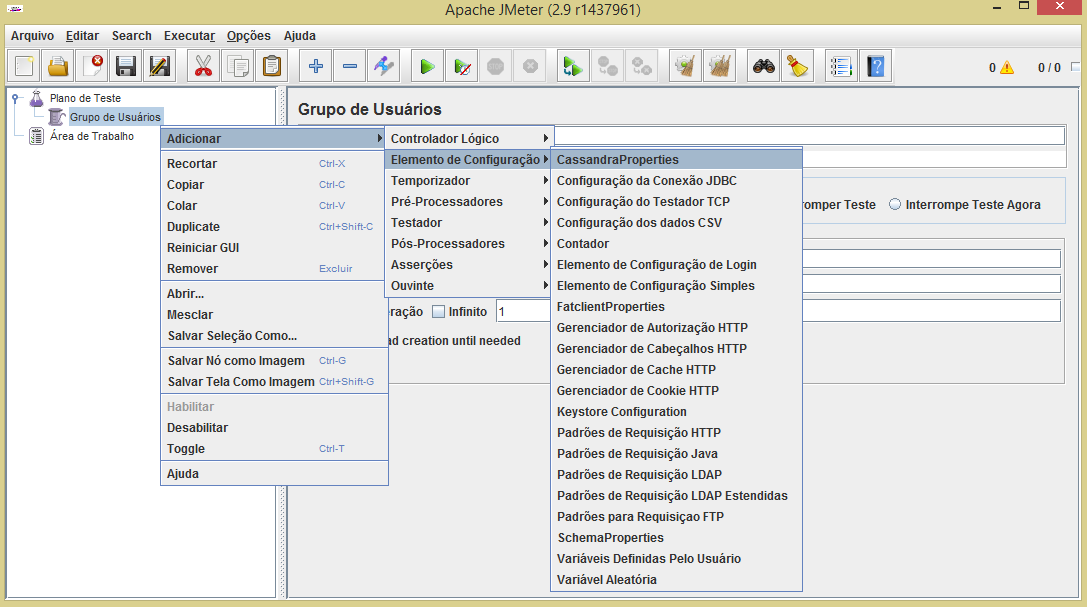
\includegraphics[scale=0.5]{imagens/cassandraprop.png}
    \caption{Propriedades da conexão com Cassandra}
    \label{fig:cassandraproperties}
    \end{figure}


\subsection{Configurando arquivo de dados CSV}

O arquivo \textit{.csv} é utilizado para simular a gravação de dados no Cassandra. As informações contidas neste arquivo são utilizadas para identificar quais variáveis serão gravadas e como elas são delimitadas. A Figura \ref{fig:csvprop}, ilustra a tela de configuração do arquivo \textit{.csv}.

   \begin{figure}[htb]
    \centering
    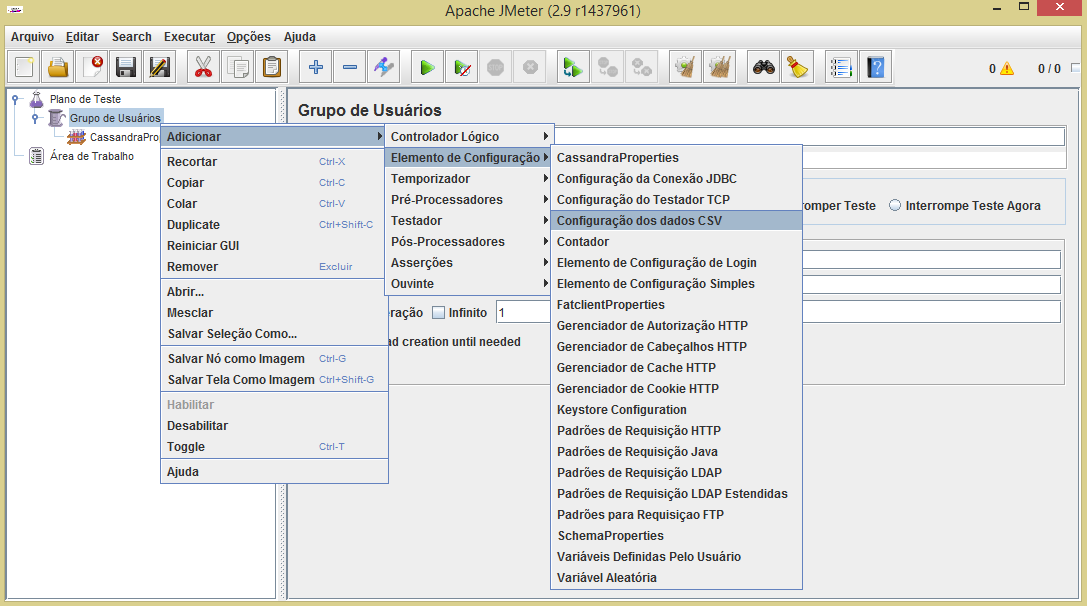
\includegraphics[scale=0.5]{imagens/csvprop.png}
    \caption{Propriedades do arquivo de dados}
    \label{fig:csvprop}
    \end{figure}

\subsection{Configurando a criação das propriedades de schema}

Através do JMeter é possível criar \textit{schemas} no Cassandra para finalidade de testes. Nesta etapa de configuração é possível definir os parâmetros: \textit{column\_family, keys\_cached, rows\_cached}, entre outros, conforme a Figura \ref{fig:schemaprop}.

   \begin{figure}[htb]
    \centering
    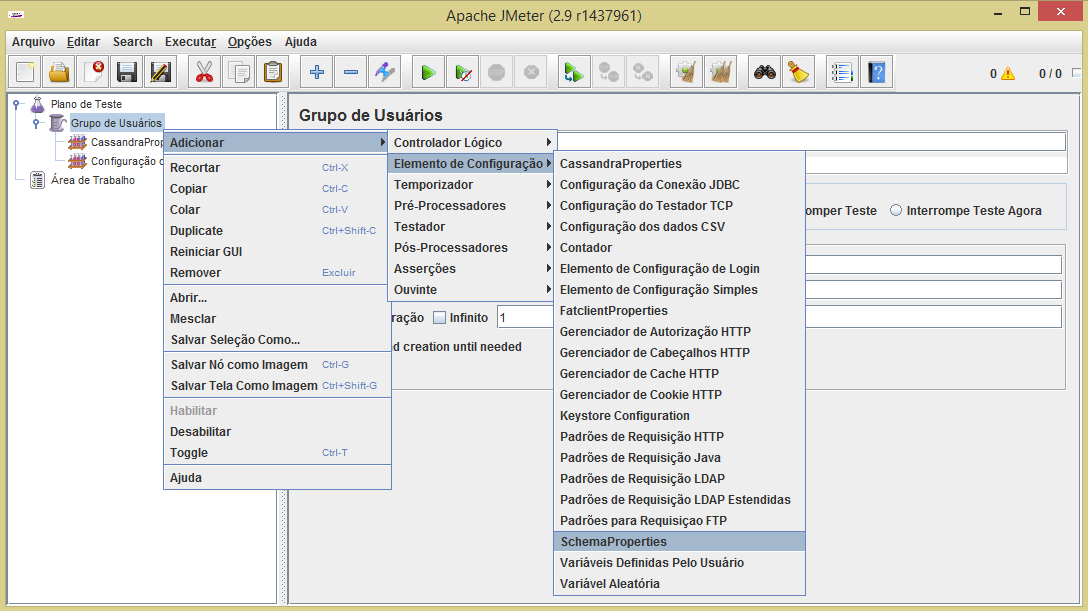
\includegraphics[scale=0.5]{imagens/schemaprop.png}
    \caption{Propriedades do \textit{schema} Cassandra}
    \label{fig:schemaprop}
    \end{figure}

\subsection{Adicionando dados ao \textit{cluster}}

Para adicionar dados ao \textit{cluster} Cassandra o JMeter faz uso de controladores chamados, genericamente, de Testadores. Existem vários tipos de Testadores, para os mais variados tipos de serviços. Para executar a operação de adição de dados ao \textit{cluster} Cassandra utilizou-se o Testador Cassandra \textit{Put}. O caminho para os controladores de requisição é: Editar/Adicionar/Testador, conforme Figura \ref{fig:cassandraput}.


   \begin{figure}[htb]
    \centering
    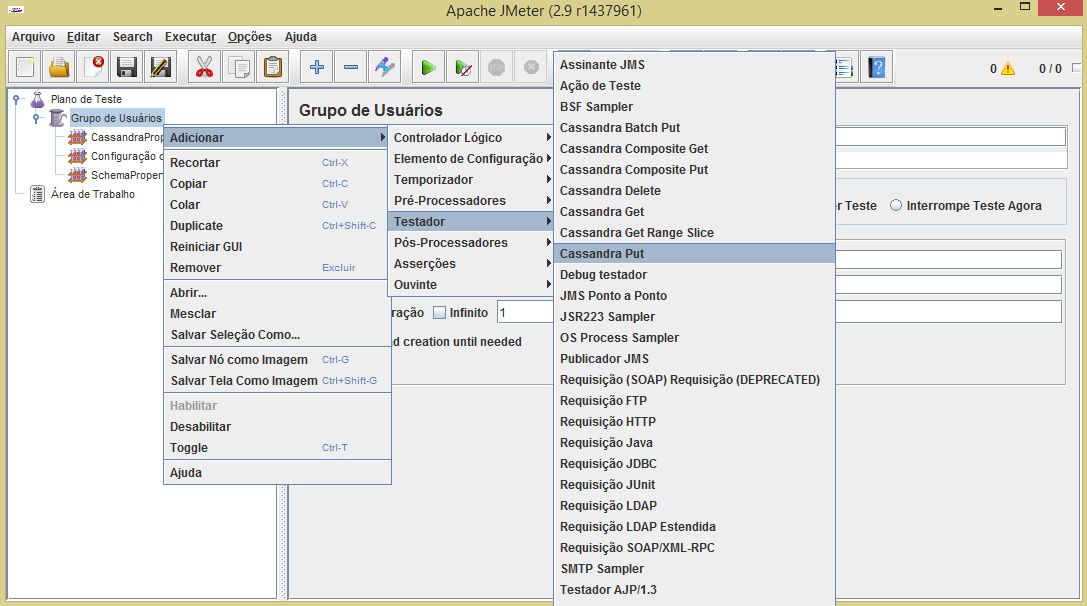
\includegraphics[scale=0.5]{imagens/cassandraput.png}
    \caption{Exemplo de gravação de dados no Cassandra}
    \label{fig:cassandraput}
    \end{figure}